\documentclass{sig-alternate-05-2015}

\begin{document}

\title{CS265 Midway Checkin}
\subtitle{Optimizing Memory Allocation Between Memtable, Cache, and Bloom Filters}
\numberofauthors{3}
\author{
\alignauthor
Mali Akmanalp\\
       \affaddr{Harvard University}\\
       \email{mea590@g.harvard.edu}
\alignauthor
A. Sophie Hilgard\\
       \affaddr{Harvard University}\\
       \email{ash798@g.harvard.edu}
\alignauthor Andrew Ross\\
       \affaddr{Harvard University}\\
       \email{andrew\_ross@g.harvard.edu}}

\date{\today}

\maketitle

\section{Introduction}
Tuning data systems is hard. Even for systems like key-value stores that only
support the most minimal API (\texttt{put} and \texttt{get}), the possibilities
are often overwhelming. The developers of RocksDB \cite{facebook:rocksdb}, a
popular and powerful key-value store, freely admit that ``configuring RocksDB
optimally is not trivial,'' and that ``even [they] as RocksDB developers don't
fully understand the effect of each configuration change''
\cite{rocksdb-tuning-guide}. Configurations must be optimized with respect to a
given \textit{workload}, which is rarely known in advance, although it is
sometimes roughly characterizable. There has been recent work \cite{monkey} in
determining the optimal memory allocation for bloom filters in terms of
worst-case analysis and with respect to a number of basic workloads, but
realistic key-value store workloads, which have been analyzed e.g. for Facebook
\cite{characterizing-memcached}, exhibit enormous complexity with respect to
time, skewness, and key repeatability.

Our goal is somewhat ambitious -- we seek to optimize not just bloom filter
memory allocation but memory allocation across the entire key-value store (to
cache, memtable, bloom filters, and possibly even fence pointers), and to do it
with respect to workloads we model as stochastic processes.

\section{Workloads}

Here are a number of basic workloads we will use to generate queries to
benchmark our key-value store, both in RocksDB and in Python simulations. For
the simpler ones, we will also attempt to predict performance and derive
optimal parameters analyitically.

\textbf{Uniform} queries will be drawn uniformly from keys $k \in
\{0,1,...,K\}$, where $K$ is a maximum key (that we explore varying). When we
draw a particular key $k_i$ for the first time, we will insert it into the
database as a write, and subsequently we will treat it as a lookup. Later we
will explore making a certain fraction of these queries into updates. The case
of uniformly distributed queries is often one in which the cache is unhelpful,
but in practice is highly unrealistic. Nevertheless, this is the scenario that
many analyses assume for calculations of big O complexity.

\textbf{Round-Robin} queries are drawn deterministically using $k_i = (i \mod
K)$, i.e. we iteratively draw each key in sequence, then repeat. This is also a
bad case for our key-value store in its default configuration; the fact that a
key has been recently written or read is actually a contraindication we will
access it again.

\textbf{80-20} queries (which are considered in \cite{monkey}) are drawn such
that 20\% of the most recently inserted keys constitute 80\% of the lookups.
This is a simple model we will be able to analyze analytically that exhibits
more realistic skew.

\textbf{Zipf} queries are distributed according to a Zipf or zeta distribution,
where the probability of a given key $k$ is $\propto \frac{1}{k^s}$, where $s
\in (1, \infty)$ describes the skewness of the distribution; in the limit
$s=1$, it is uniform with $K=\infty$. Zipf-distributed queries are considered
in \cite{art} as another simple proxy for realistically skewed queries.

\textbf{Discover-Decay} queries are distributed according to the following
stochastic process, inspired by the Chinese Restaurant process \cite{crp} but
with time decay: with every passing time increment $\Delta t \sim
\textrm{Expo}(\lambda_t)$, $n \sim \textrm{Pois}(\lambda_n)$ new keys are written to the
key-value store, which each have an inherent popularity $\theta_i \sim
\textrm{Beta}(a_\theta,b_\theta)$ with a random decay rate $\gamma_i \sim
\textrm{Beta}(a_\gamma,b_\gamma)$ that determines the exponential rate at which they
become less popular. The probability of drawing each $k_i$ is given by
$p(k_i,t) \propto \theta_i\gamma_i^{t-t_i}$, where $t$ is the current time and
$t_i$ is when the key was inserted. At each time step we sample $N$ keys from
$\textrm{Mult}(\{p(k_i,t)\})$. This stochastic process is somewhat arbitrary and we
hope to make it more realistic, but it does capture many of the essential
behaviors we know characterize key-value stores: new keys are constantly
inserted, some keys are much more popular than others, and the popularity of
most keys decays over time. The nonparametric nature of this stochastic process
may make inference difficult, and we also hope to enhance it to make it more
well-suited to realistic workloads (e.g. that exhibit daily periodicity), but
it seems much more able to simulate the richness of realistic queries than many
of the other models.

\section{Simulations}

We implemented a basic simulator of an LSM tree in Python \cite{lsmulator},
which simulates how an LSM tree with a variably sized cache, memtable, disk
layers, and bloom filters performs for an aribtrary sequence of queries. In
particular, we are able to simulate how often we are forced to access data on
disk (the main performance bottleneck for an LSM tree) and how often we can
respond with data in memory. So far, results suggest that the same LSM tree
architecture performs very differently under different query distributions
(Figure \ref{fig:sametree-diffqs}), and that different LSM tree architectures
perform very differently under the \textit{same} query distribution (Figure
\ref{fig:sameqs-difftree}). We are working on an optimization procedure to find
the best architecture for a given set of queries.

\begin{figure}[!htb]
\begin{center}
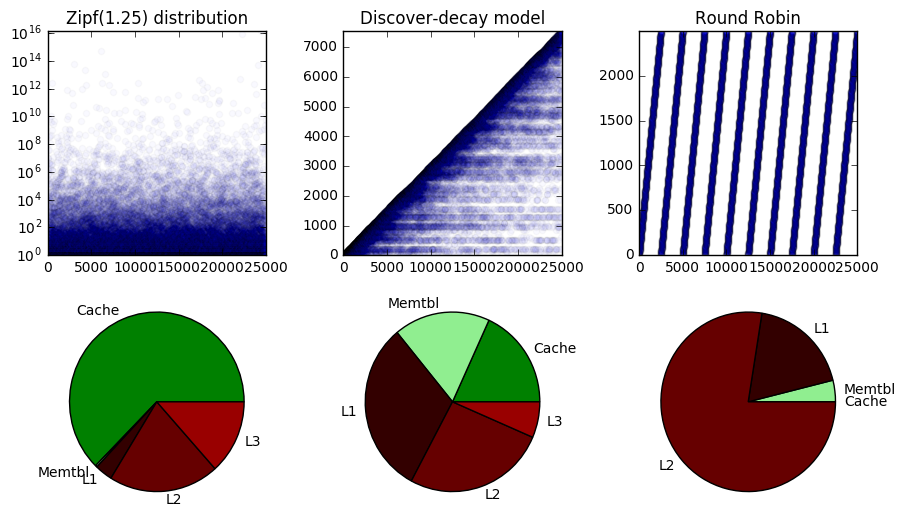
\includegraphics[width=9cm]{sametree-diffqs.png}
\end{center}
\caption{The same LSM tree architecture (a 25-element cache, 100-element
memtable, 5x layer ratio, and 10-bit bloom filters with 5 hash functions)
performs very differently for different query distributions. Memtable and cache
hits (in green) are fast, whereas accesses to the layers (in red) are slow. For
the Zipf workload, the cache is much more useful than the memtable, while the
situations are reversed for the Round-Robin workload. Both are useful in the
discover-decay case.}
\label{fig:sametree-diffqs}
\end{figure}

\begin{figure}[!htb]
\begin{center}
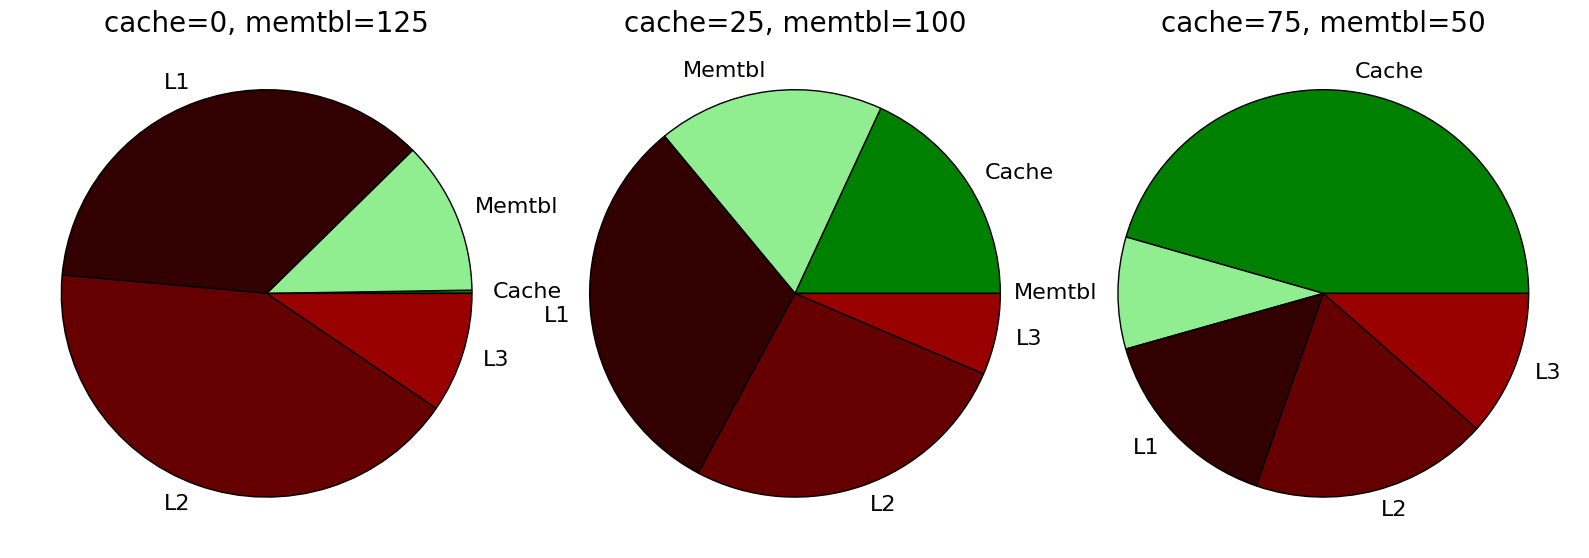
\includegraphics[width=9cm]{sameqs-difftree.png}
\end{center}
\caption{Performance results for different LSM tree architectures on the
discover-decay workload. Note that for this time-dependent workload, both the
cache and the memtable are useful, but finding the best ratio may require
optimization.}
\label{fig:sameqs-difftree}
\end{figure}

\section{Benchmarking}

So far, we've succeeded in getting basic benchmarks for RocksDB running and
identifying which configuration parameters to vary. Our next step will be
to generate queries in RocksDB format that correspond to our probabilistically
modeled workloads, run them against RocksDB under different configurations
that correspond to simulation parameters, and see if results match at least
qualitatively.

\section{Modeling}

Ideally, instead of resorting to simulation, we should be able to analytically compute the expected cost (in disk reads) of reading an element from our LSM tree. The following sections show some of our initial results under different assumptions about the query distribution. By the end of this project, we hope to show concordance between these results, simulations, and experiments with RocksDB.

\subsection{Uniform query distribution}

\noindent Assuming we have
\begin{itemize}
  \item $n_t$ total items in the database
  \item $n_c$ items that fit in cache
  \item $n_m$ items that fit in memtable
  \item a ratio $R$ between layers of LSM tree such that
  \item $L1 = R * n_m$, $L2 = R^2 * n_m$, and so on,
\end{itemize}

\noindent then we can solve for $j$, the total number of layers required to store all the data: \\
$$n_t = n_m * \frac{1-R^j}{1-R},\  j = \frac{\log(1-n_t*\frac{1-R}{n_m})}{\log R}$$

The average cost of a write remains the same as for the basic LSM tree case:
$$
\text{write cost} = \textrm{log}_{R} \frac{n_t}{n_m}
$$

The average cost of a read must be considered probabilistically over all possible locations of the read item, in this case assuming a uniformly random distribution of reads:
\begin{itemize}
\item Probability that read is in memtable $= p(\text{MT}) = \frac{n_m}{n_t}$
\item Probability that read is in cache $= p(\text{cache}) = \frac{n_c}{n_t}$
\item Probability that read is in L1 but not in cache $= p(L1)$ $$= \frac{n_m * R - \frac{n_m * R}{n_m * \frac{1-(R^j-1)}{1-R}} * n_c}{n_t}$$
\end{itemize}
where the numerator is the number of items $n_m * R$ that are in the first layer minus the proportion of items from that layer that are probabilistically in the cache already: $$\frac{n_m * R}{n_m * \frac{1-(R^j-1)}{1-R}} * n_c$$
and finally where the $R^j -1$ comes from the fact that items already in memtable (L0) are not allowed to occupy the cache.

Therefore, given a uniform query distribution, the full expected cost in disk reads of a read is
$$E[C_{\text{uniform}}] = p(\text{MT}) * 0  + p(\text{cache}) * 0 + \sum_{i=1}^j p(L_i) * i$$
$$= \sum_{i=1}^j \frac{n_m * R^i - \frac{n_m * R^i}{n_m * \frac{1-(R^j-1)}{1-R}} * n_c}{n_t}  * i$$

\subsection{Skewed Reads (80-20)}

Now consider the case for skewed reads, where we say $d_{hf}$ ($d_{lf}$) percent of the data ($hf \equiv$ high-frequency) receives $r_{hf}$ ($r_{lf}$) percent of the reads (where $d_{hf} + d_{lf} = 1$ and $r_{hf} + r_{lf} = 1$). On average, we can assume that the cache contains $r_{hf} * n_c$ items from $d_{hf} * n_t$ and $r_{lf} * n_c$ items from $d_{lf} * n$. Then the expected cost of a read is dependent on whether the data item being read is in $d_{hf} * n_t$ or $d_{lf} * n$ as the probability of a cache hit varies.\\ \\
Concretely, consider where we have 3 levels and 800 total items with a cache of size 10 and a ratio of 2  (for L0=100, L1 = 200, L2 = 400 items), with $d_{hf} = .2$ and $d_{lf} = .8$ and $r_{hf}$ = .8 and $r_{lf}$ = .2, which matches the scenario considered in \cite{monkey}. Then the cache, on average, contains 8 items from $d_{hf} * n$ and 2 items from $d_{lf}*n$. If we execute a read on one of the 200 items in $d_{hf}$, then, there is a $\frac{8}{200}$ chance that that item is in the cache. If we execute a read on one of the $200*\frac{1}{4} = 50$ items of  $d_{hf} * n_t$ in L1, we expect that $\frac{2}{6} * 8$ of those items would have actually been found already in cache, as this level contains $\frac{2}{6}$ of all of the items not in the memtable. Then the probability that a read is found in L1 is the proportion of the $d_{hf} * n_t = 160$ items that will reside in L1 but not in the cache, which is $\frac{40 - \frac{2}{6} * 8}{160}$. \\ \\
Just limiting ourselves to high-frequency data, we see that:
\begin{itemize}
  \item Probability that read is in memtable $= p(\text{MT}_{hf}) = \frac{n_m*d_{hf}}{d_{hf} *n_t}$
  \item Probability that read is in cache $= p(\text{cache}_{hf}) = \frac{r_{hf} * n_c}{d_{hf} * n_t}$
  \item Probability that read is in $L_i$ but not in cache $= p(L_{i,hf})$ $$ = \frac{n_m * R^{i}*d_{hf} - \frac{n_m * R^{i}}{n_m * \frac{1-(R^j-1)}{1-R}} * r_{hf} * n_c}{d_{hf} * n_t} $$
\end{itemize}

This gives us the final expected cost of reading high frequency items:
$$
\begin{aligned}
E[C_{\text{skewed}, hf}]
& = p(\text{MT}_{hf}) * 0  + p(\text{cache}_{hf}) * 0 + \sum_{i=1}^j p(Li_{hf}) i \\
& = \sum_{i=1}^j \frac{n_m * R^{i}*d_{hf} - \frac{n_m * R^{i}}{n_m * \frac{1-(R^j-1)}{1-R}} r_{hf} n_c}{d_{hf} n_t} i
\end{aligned}
$$

The expected cost of reads for low-frequency items can be enumerated analogously, and combining the expectation of reads in $d_{hf}$ and $d_{lf}$, we obtain
$$
E[C_{\text{skewed}}] = r_{hf} * E[C_{\text{skewed}, hf}] + r_{lf} * E[C_{\text{skewed}, lf}],
$$

which is the expected number of lower layer accesses per read on a workload where $d_{hf}$ percent of the data receives $r_{hf}$ of the reads.

\subsection{Bloom Filters}

The previous analysis hasn't yet accounted for the presence of Bloom filters, which reduce the likelihood we will unnecessarily access a lower layer. For a Bloom filter of $k$ bits with $h$ independent hash functions $h_1, h_2,...h_h$, the probability that a given bit is still set to 0 after inserting $n$ keys is 
$$
(1 - \frac{1}{k})^{n*h}
$$
Then the probability of a false positive is 
$$
(1- (1 - \frac{1}{k})^{n*h})^h \approx (1 - e^{-hn/k})^h
$$

We can minimize this over $h$ to find the optimal number of hash functions, which is $h = \mathrm{ln}(2) * \frac{k}{n}$. Assuming that this is the number of hash functions $h$ we will use, the probability of a false positive as a function of the number of bits is then 
$$
(1 - e^{-\mathrm{ln}(2)*k/n*n/k})^{\mathrm{ln}(2) * \frac{k}{n}} = (\frac{1}{2}) ^ {\mathrm{ln}(2) * \frac{k}{n}} \approx (.6185) ^  {\frac{k}{n}}
$$

For an item in any any level $L_i$ of the LSM tree with $i \geq 2$ we can reduce the expected cost of accessing that item from $i$ by the number of Bloom filter negatives at any level $j<i$. \\ \\
Then the expected cost of accessing an item at $L_i$ is  $$\sum_{j=1}^{i-1} p(fp_j) * 1 + 1$$
Where $p(fp_j)$ is the probability of a false positive for that key at level $j$ and 1 is the cost of actually accessing the item at level $i$ assuming fence pointers that lead us to the correct page.

\subsection{Variable Cache, Constant Layers}

Now we want to analyze what happens when we vary the proportion of memory allocated to the cache and the memtable. Given a fixed memory size $n_v$, we first consider the simplification of assuming a constant layer structure. Of course, in general a larger memtable will allow for larger layers, affecting both read and write performance. Let $n_l$ be the size of the first layer when $n_v = n_m$ (all memtable) and $n_c =n_v - n_m$.\\ \\
\textbf{Uniform Case:} \\
%if we assume some fixed base layer size $n_l$, which is the size of the memtable if it exists.
Consider the formula used earlier:
$$
p(\text{MT}) * 0  + p(\text{cache}) * 0 + \sum_{i=1}^j p(L_i) * i 
$$

In the extreme case where $n_m=0$ (\textbf{no memtable}), the formula in the numerator of the sum simplifies to be over $n$ the total number of items, as there is no memtable layer and the probability of the first layer now has a cost of 1. However, we now have to add a number of items to each level of the tree that sum to the amount that were in L0. We add them as a geometric series per layer to maintain the structure
$$
\sum_{i=i}^{j} \frac{(n_l) * R^{i} + \frac{(n_l) * R^{i}}{n_t} * n_v - \frac{(n_l) * R^{i}}{n_t} * n_v}{n_t} * (i)
$$
The two latter terms cancel and we are left with
$$
\sum_{i=1}^j \frac{(n_l) * R^i}{n_t} * i 
$$
In the extreme case of \textbf{no cache}, 
$$
\sum_{i=1}^j \frac{(n_l) * R^i}{n_t} * i 
$$
And we can see that this is in fact the same result as the no memtable case. \\ \\
In general, for any selection of $n_m$ and $n_c$ we have
\begin{multline}
\sum_{i=1}^j \frac{(n_l) * R^i - \frac{(n_l) * R^i}{(n_l) * \frac{1-(R^j-1)}{1-R}} * (n_v-n_m)}{n_t} \\+
\frac{\frac{(n_l) * R^i}{(n_l) * \frac{1-(R^j-1)}{1-R}} * (n_v-n_m)}{n_t} * i 
\end{multline}
and so with a random workload, the choice is irrelevant \textit{assuming a constant number of layers}. In actuality, with a larger memtable we will be able to decrease the total number of layers needed. \\
\\
\textbf{Skewed Reads (80-20) Case:}\\
Now consider the case for skewed reads, where we say $d_{hf}$ ($d_{lf}$) percent of the data receives $r_{hf}$ ($r_{lf}$) percent of the reads (where $d_{hf} + d_{lf} = 1$ and $r_{hf} + r_{lf} = 1$). On average, we can assume that the cache contains $r_{hf} * n_c$ items from $d_{hf} * n_t$ and $r_{lf} * n_c$ items from $d_{lf} * n$. \\ \\
In the extreme case of \textbf{no cache}, the result will be as above. \\ \\
In the extreme case of \textbf{no memtable}, the expected cost of a read is dependent on whether the data item being read is in $d_{hf} * n_t$ or $d_{lf} * n$ as the probability of a cache hit varies.\\
For data in $d_{hf} * n$, \\ \\
Probability that read is in cache:
$$\frac{r_{hf} * n_c}{d_{hf} * n_t} = p(\text{cache}_{hf})$$ \\
Probability that read is in $L_i$ but not in cache: 
\begin{multline}
\frac{n_l * R^{i}*d_{hf} - \frac{n_l * R^{i}}{n_t} * r_{hf} * (n_v)}{d_{hf} * n_t} \\+ \frac{\frac{n_l * R^{i}}{n_t} *d_{hf} *(n_v)}{d_{hf} * n_t}  \\= \frac{n_l * R^{i}*d_{hf}+ \frac{n_l * R^{i}}{n_t} * (d_{hf}-r_{hf})* n_v}{d_{hf} * n_t} = p(Li_{hf}) 
\end{multline} \\
Expected cost of read on item in $d_{hf}$: \\
$$E[C_{hf}]= p(\text{cache}_{hf}) * 0 + \sum_{i=1}^j p(Li_{hf}) * i$$\\
$$
= \sum_{i=1}^j \frac{n_l * R^{i}*d_{hf}+ \frac{n_l * R^{i}}{n_t} * (d_{hf}-r_{hf})* n_v}{d_{hf} * n_t}  * i
$$ \\
From this equation we can see that the probability (and thus the expected cost) is increasing in $d_{hf}$ and decreasing in $r_{hf}$. This makes sense, as for many reads (high $r_{hf}$) on a small amount of data (low $d_{hf}$) we would expect frequent cache hits. \\ \\
For general memtable/cache allocation, probability that read is in $L_i$ but not in cache: 
\begin{multline}
\frac{n_l * R^{i}*d_{hf} - \frac{n_v * R^{i}}{n_l * \frac{1-(R^j-1)}{1-R}} * r_{hf} * (n_v - n_m)}{d_{hf} * n_t} \\+ \frac{\frac{n_v * R^{i}}{n_l * \frac{1-(R^j-1)}{1-R}} *d_{hf} *(n_v - n_m)}{d_{hf} * n_t}  = p(Li_{hf})
\end{multline}

\subsection{Future Modeling Work}

What we have done so far is to analytically compute basic quantities (like the
expected cost of individual reads) as a function of LSM tree attributes for
basic query distributions. Once we extend this analysis to allow the number of
layers to vary with the memtable size, we should be able to directly compare
these analytic results to simulation and experimental benchmarks, and then
finally attempt to derive optimal LSM tree parameters.

\section{Bringing it all together}

Once we have analytic and simulated predictions of optimal RocksDB
configurations that match benchmarking experiments, the final step will be to
consider whether we can implement adaptive updating in RocksDB to optimize
performance on the fly. We are considering several options, including on-the-fly
inference and maintaining a small number of fixed parameter settings that we can
dynamically decide between to simplify the problem.

Overall, however, we believe even being able to determine the optimal LSM tree
architecture in theory (based on a deep and accurate characterization of the
workload) will be a useful contribution.

\bibliographystyle{abbrv}
\small
\bibliography{bibliography}

\end{document}
